\newcommand{\auteur}{Stalder Lawrence, Pombo Dias Miguel, Cotza Andrea Roberto, \\
	
	Verdasca Jimmy, Clavier Tony \& Guillod Maxime}
\newcommand{\cours}{GEN}
\newcommand{\ecole}{IL --- TIC --- HEIG-VD}
\newcommand{\domaine}{PDG}
\newcommand{\titre}{WordOn Desktop}

\documentclass[a4paper,12pt]{article}
%
\author{\auteur}
\title{\titre}
\date{\today}

\usepackage[frenchb]{babel}
\usepackage{fancyhdr}
\usepackage{graphicx}
\usepackage{amsmath}
\usepackage{listingsutf8}
\usepackage{color}
\usepackage{enumerate}
\usepackage[utf8]{inputenc}
\usepackage[T1]{fontenc}
\usepackage{float}
\usepackage{geometry}
\usepackage{amssymb,mathtools,pifont}
\usepackage{enumitem}
\usepackage{xspace}
\usepackage{appendix}
% Liens
\usepackage[hyphens]{url}
\usepackage{hyperref}
\geometry{verbose,tmargin=2.5cm,bmargin=2.8cm,lmargin=1.8cm,rmargin=1.8cm}
\selectlanguage{frenchb}
\frenchbsetup{StandardLists=true}
\DeclareGraphicsExtensions{.pdf,.png,.jpg}
\setlength\parindent{0pt}
\setlength{\parskip}{0.7em}

\usepackage{listings}
\lstset{
	breaklines=true, 
	basicstyle=\scriptsize,
	inputencoding=utf8/latin1,
	extendedchars=true,
	numbers=left,
	firstnumber=1,
	numberfirstline=true, 
	language=Java,
	keywordstyle=\color{blue}\ttfamily,
	stringstyle=\color{red}\ttfamily,
	commentstyle=\color{black}\ttfamily
}


% headers & footers
\pagestyle{fancy}

\lhead{\domaine}
\rhead{\titre\space
\includegraphics[scale=0.12]{logo/logo.png}}

\renewcommand{\footrulewidth}{0.4pt}% default is 0pt
\lfoot{\auteur}
\cfoot{}
\rfoot{\thepage}

%%%%%%%%%%%%%%%%%%%%%%%%%%%%%%%%%%%%%%%
%%%%%%% BEGIN DOCUMENT
%%%%%%%%%%%%%%%%%%%%%%%%%%%%%%%%%%%%%%%

\begin{document}
	\clearpage\maketitle
	\thispagestyle{empty}
	
	\maketitle
	\begin{figure}[h!]
		\centering
		
\includegraphics[scale=1]{logo/logo.png}
	\end{figure}
	\newpage
	
	% % Entete première page
	% \thispagestyle{empty}
	% %
	% \noindent \cours \hfill \ecole{} \newline
	% \noindent \auteur \hfill \today \newline
	% \hrule
	% \vspace{7mm}
	% \noindent {\large \bf \domaine } \hfill \titre {\large \bf }\\[3mm]
	% \hrule
	
	\tableofcontents
	
	\listoffigures
	
	% On a pas de tableau
	% \listoftables
	
	\newpage
	
	\section{Description générale du projet}
	\subsection{Cadre / contexte}
	Ce projet a lieu dans le cadre du cours PDG à la HEIG-VD à Yverdon-les-Bains dans le cadre de notre dernière année de bachelor en informatique.
	
	\subsection{But(s) visé(s)}
	A l'issue de ce cours ainsi que de ce projet, nous devrons être capables de spécifier, coder ainsi que tester une application de taille importante.
	
	De plus, ce projet nous apprend à acquérir par nous-mêmes des connaissances sur des nouveaux sujets en fonction de nos besoins lors de la création de notre application. 
	
	Il y a également toute la gestion de la problématique d'un projet en équipe, en groupe de 6 personnes. En effet, ceci demande une très bonne coordination entre chaque membre afin de bien séparer le travail et de faire en sorte d'avoir un projet unique et harmonieux à terme. Ceci nous demandera d'utiliser plusieurs outils spécifiques.
	
	\section{Description du jeu sur Smartphone}
	\subsection{Fonctionnalités offertes}
	\subsubsection{Inscription}
	\subsubsection{Mode normal}
	\subsubsection{Mode tournoi}
	\subsubsection{Bonus}
	
	\subsection{Règles du jeu}
	\subsubsection{Mode tournoi}
	
	\section{Jeu sur PC}
	\subsection{Introduction}
	% Notre version sur PC, de part de la résolution ainsi que de la taille de nos écrans, peut bénéficier d'une interface bien plus complète (concentrée sur la même fenêtre) que la version mobile. Par exemple, le lobby, la partie séléctionnée ainsi que le chat de la partie courante s'affiche sur la même fenêtre. 
	
	\subsection{Interface}
	L'interface utilisateur à été revue et optimisée pour l'affichage sur ordinateur en raison de la taille d'écran ainsi que sa résolution plus importante. \\
	Cependant, nous avons voulu garder la patte graphique du jeu original sur mobile en reprenant les codes couleurs et les éléments visuels spécifique au jeu.
	
		\subsubsection{Connexion et inscription}
		
		\begin{figure}[h]
			\centering
			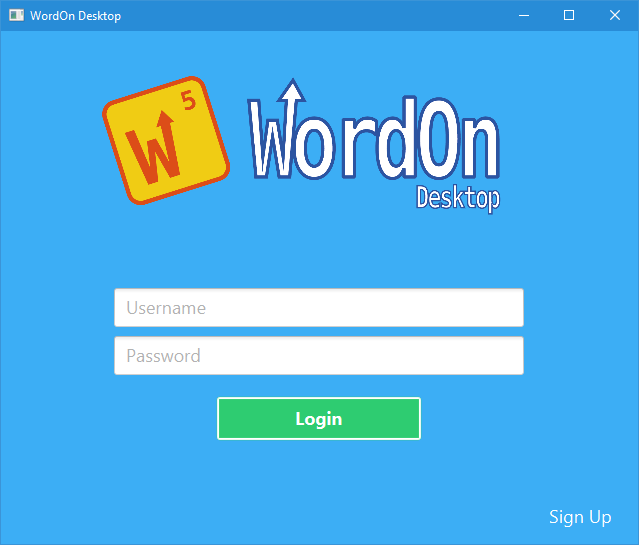
\includegraphics[width=0.4\linewidth]{img/signin.jpg}
			\caption{Fenêtre de connexion}
		\end{figure}
	
		\begin{figure}[h]
			\centering
			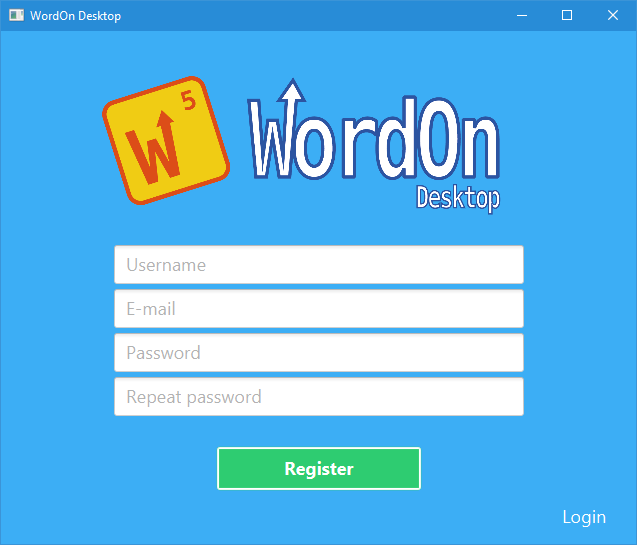
\includegraphics[width=0.4\linewidth]{img/signup.jpg}
			\caption{Fenêtre d'enregistrement}
		\end{figure}
		
		\subsubsection{Jeu}
		La taille plus importante de l'écran nous permet nottament d'afficher le lobby, la partie séléctionnée ainsi que le chat correspondant à la partie en cours. Ceci rend l'expérience de jeu plus adaptée à l'environnement desktop et permet une meilleure vue de toutes les parties en cours.
		
		\begin{figure}[h]
			\centering
			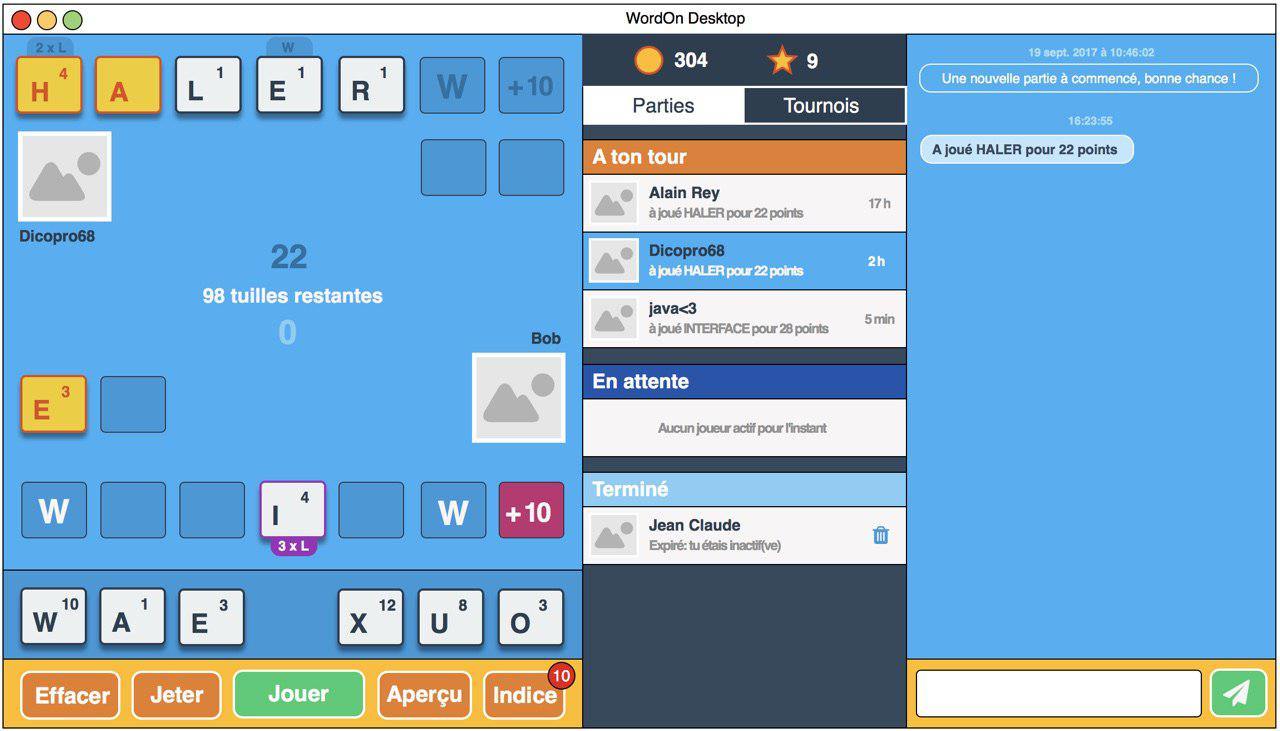
\includegraphics[width=0.6\linewidth]{img/main.jpg}
			\caption{Interface principale}
		\end{figure}
		
	\subsection{Conception}
	
	\subsection{Implémentation}
	\subsubsection{Dictionnaire}
	
	\subsubsection{Algorithme tirage aléatoire}
	
	\subsubsection{Communication}
	
	\subsection{Tests}
	\subsubsection{Bug connu}
	
	\subsubsection{Fonctionnalité pouvant être ajoutée}
	
	\section{Technologie utilisée}
	\subsection{JUnit}
	JUnit est un framework Java permettant de faire des tests unitaires. Ce dernier comporte de nombreuses méthodes afin d'automatiser les tests, et est utilisé par \hyperref[maven]{Maven}.\\
	Il permet par exemple de comparer des valeurs attendues de méthode avec ce que l'on reçoit vraiment. On peut tester l'intégralité des communications avec un tel système. De plus, il permet de s'assurer que même lors du développement d'un tel projet, les méthodes et fonctions codées précédemment n'ont pas un comportement différent en fonction du contexte d'appel. 
	
	\subsection{JavaFX}
	JavaFX est une bibliothèque d'interface graphique. Nous l'avons utilisée, avec l'aide de SceneBuilder\footnote{\textbf{SceneBuilder} : \href{http://gluonhq.com/products/scene-builder/}{gluonhq.com/products/scene-builder/}} qui permet de créer des interfaces graphiques de manière intuitive et visuelle. \\
	Cette librairie permet également de gérer tout ce qui est des interactions avec notre environnement graphique à l'aide de \textit{listener} qu'on peut lier à nos briques, nos éléments graphiques. 
	
	\subsection{GitHub}
	GitHub\footnote{\textbf{GitGub} : \href{http:/github.com}{github.com}} utilise la technologie git qui permet de gérer les fichiers d'un projet sur différentes branches, tout en faisant du versionning en ligne. Il offre également la possibilité de gérer les issues avec un système communautaire (du groupe) pour la résolution, mais également une gestion de planning et d'attribution de tâches. \\
	Ceci nous a permis de bien pouvoir séparer le travail et les parties, pour ensuite, une fois validé par les tests, les intégrer dans notre projet, soit sur la branche master. 
	
	\subsection{Apache Maven} \label{maven}
	Maven est un outil de gestion et d'automatisation de projet Java. Il permet notamment d'automatiser les dépendances de notre projet en téléchargent automatiquement les librairies utilisées par les autres membres du groupe. Il permet également de tester le projet en lançant tout les tests de notre projet avant de le compiler afin de garantir du bon fonctionnement de ce dernier. 
	
	\subsection{Docker}
	
	\section{Conclusion}
	
	\section{Annexes}
	
	
\end{document}

